\setcounter{page}{1}
\chapter{Introduction}
\label{intro}

As the title of this thesis suggests its background is twofold. On one hand it is founded on transition rate theory over fluctuating barriers, on the other hand it is based on the theory of diffusion controlled reaction rates. 
\vspace{-.3 cm}
\section{Transition Rate Theory} 

The subject of transition rate theory has been studied empirically since the mid 18th century by Van't Hoff \cite{hoff1884} and Arrhenius \cite{arrhenius1889}. But not before 1940 it was built upon a thorough theoretical foundation when Kramers published his celebrated paper on ``Brownian Motion in a Field of Force and the Diffusion Model of Chemical Reactions'' \cite{Kramers1940}.  He described the escape from a metastable state as a noise assisted reaction, and derived the well known Kramers reaction rate from the strong friction limit of the description of Brownian motion dynamics.
Building upon Kramers results, Doering and Gadoua \cite{Doering1992} were the first to investigate the case in which the potential defining the metastable state in an escape problem is not constant but subject to fluctuations. Their setup as depicted in figure \ref{Gadoua} consisted of a piecewise linear barrier between \\[0.3 cm] \begin{minipage}[t]{0.62 \textwidth}
        \captionof{figure}{Sketch of the system investigated in Doering\&Gadouas 1992 paper \cite{Doering1992} on Resonant Activation.  Two states between reflecting walls at $L$ and $-L$ are separated by a piecewise linear potential. The Potential fluctuates between states of different height $E_+$ and $E_-$ subject to symmetric dichotomous noise with rate $\gamma$. The trajectory of the thermally activated particles is denoted by $X(t)$. They exhibit a minimum in mean first passage time across the barrier depending on the rate of barrier fluctuations.\label{Gadoua}}
\end{minipage}\begin{minipage}[t]{0.38 \textwidth}
    \begin{figure}[H]
         \includegraphics[width = 1 \textwidth]{plots/Gadoua.png}
    \end{figure}
\end{minipage} 

two reflecting walls that fluctuates between two distinct states in height as a Markov process with rate $\gamma$.

 They discovered an effect that they called \emph{resonant activation} which describes a local minimum in mean first passage times depending on the barrier fluctuation rate emerging from the interplay of the timescales of barrier crossing and barrier fluctuations. \\
In the following years this effect has drawn significant interest from the community and has been thoroughly studied for several classes of potentials and a variety of processes describing its fluctuations \cite{Zurcher1993, Pechukas1994, Reimann1995, Reimann1995a}. The progress on the topic has been nicely reviewed by Peter Reimann and Peter H\"{a}nggi in 1997 \cite{Reimann1997}.

\section{Diffusion Controlled Reactions}
Reaction rate theory has been studied in physics, chemistry and biology since the early 19th century. All latter inquiries on the topic are founded on the pioneering work of Marian von Smoluchowski from 1916 and 1917 who held a series of talks \cite{Smoluchowski1916} describing the motion of Brownian particles in solution and used it to describe the coagulation of gold particles \cite{Smoluchowski1917a}. He thereby obtained the famous Smoluchowski reaction rate of ideal Brownian particles of radius $R_p$ being absorbed in a spherical sink of radius $R_s$:\\
\begin{equation}
    K_S = 4 \pi D R \rho_0 \nonumber
    \label{Ksintro}
\end{equation}
where $D = D_p + D_s$ is the relative bulk diffusion constant, $\rho_0$ the bulk density of the Brownian particles and $R = R_p + R_s$ is the encounter distance. This result is valid for noninteracting reactants in ideal infinitely diluted solution. \\ 
Since these conditions strongly restrict the applicability of this general result to real world problems, the theory of diffusion controlled reactions has been widely extended in the course of the 19th century.\\
In the 1940s Debye \cite{Debye1942} modified this basic model to include interactions between Brownian particle and the sink when he investigated the rate for diffusion limited reactions between charged particles in solution. Thereby he obtained the so called Smoluchowski-Debye reaction rate:
\begin{equation}
    K_D = \rho_0\left\{\int_{R_s}^{\infty} \frac{\exp \left[ \frac{U(r')}{K_B T}\right]}{4 \pi D(r') r'^2} \rm d r' \right\}^{-1} \nonumber
    \label{Kdintro}
\end{equation}
in which $D(r)$ is the spatially dependent diffusion profile, $U(r)$ is the interaction potential, $\rho_0$ is the bulk density of the particles and $R_s$ is the encounter radius of the different particle species. \\
Debye's formula is widely applied, in e.g. heterogeneous catalysis, polymer chain growth kinetics, colloid or crystal growth and enzyme ligand binding \cite{hawker2001new, hansen2002robust, aizenberg1999control, achilias1992development, wisanrakkit1990glass, berg1985diffusion, kuo1974studies, richter1974, alberty1958, Wu2012a}. However, in most of these applications the reaction at the absorbing sink is not infinitely fast but happens with a finite rate $K_A$.The process is thus governed by both, a kinetic rate $K_D$ arising from mass transport by diffusion and an interaction rate $K_A$ that is given by the particular reaction at the sink. In this case the effective rate of the reaction turns out to be given by:
\begin{equation}
    K_{eff} = \frac{K_D K_A}{K_D + K_A}.
    \label{KeffIntro}
\end{equation}
This expression serves neatly to explain the term \emph{diffusion controlled} reactions. Depending on the ratio of $K_A$ and $K_D$ the process is either limited by the interaction reaction ($K_A \gg K_D$) such that $K_{eff} \approx K_A$ or by mass transport ($K_A \ll K_D$) such that $K_{eff} \approx K_D$. The former case is called ``reaction controlled'' whereas the latter is called ``diffusion controlled''. \\

To further extend the applicability of diffusion controlled reaction theory a variety of effects arising from finite densities and particle interactions have been taken into account. There are corrections due to hydrodynamic interaction between mutually approaching particles \cite{Friedman1966, Wolyes1976}, corrections due to combined hydrodynamic and hard sphere interaction for dilute but finite substrate concentration \cite{Dzubiella2005} as well as effects arising from crowding when substrate particles that are approximated as hard spheres occupy up to 30\% -40\% of the available volume \cite{Dorsaz2010}. Other generalizations include situations where there are multiple sinks competing for the substrate \cite{Reck1968a, Reck1968b} or setups where the reaction at the sink is limited to a certain reactive patch that covers only a fraction of its surface \cite{schmitz1972role, schurr1976, shoup1981diffusion, shoup1982role}. \\
Most of these effects have in common that they result in one of two types of corrections to the original Smoluchowski Debye problem. They can either be described by spatially dependent diffusion profiles or tensors, or they can be mapped to potentials of mean force describing an effective interaction between the species involved. In both cases the quantities describing the effect are constant in time.
\newpage
\section{The Importance of Fluctuations}
One of the key motivations for the introduction of fluctuating quantities in the field of diffusion controlled reactions was the following: in 1978 A. Szabo \cite{Szabo1978} observed that the rate of oxygen binding by hemoglobin is about an order of magnitude slower than what one would expect if it was solely diffusion controlled. It was known from previous studies that the binding site of the hemoglobin protein is blocked by certain side chains that would prohibit oxygen from binding if they were in their equilibrium position \cite{perutz1966x, muirhead1967structure}. Therefore he reasoned that these side chains would fluctuate between different states that either allowed or inhibited oxygen binding and that would therefore act as a gate that stochastically opens and closes in time. \\ In 1982 Szabo et al. described this so-called gating process in the framework of diffusion controlled reactions \cite{Szabo1982}. To make use of the  picture of Brownian particles diffusing around an absorbing sink, the sink was no longer considered to be ideal but was taken to fluctuate between different states of surface reactivity. The analytic work in this thesis is to some extent inspired by the methods they employed to treat this problem. \\
In terms of equation \eqref{KeffIntro} the fluctuating quantity in gating problems is the surface or encounter reactivity $K_A$. Unfortunately in many problems it is not (only) the encounter reactivity of the reactants that is fluctuating but (also) the interaction between the species involved. This has profound effects on the kinetic rate $K_D$. \\
One recent example where fluctuations have been suggested to play an important role are thermosensitive yolk-shell nanoparticles studied by Wu et al. \cite{Wu2012a}. They consist of a reactive Au nanoparticle encapsulated in a thermosensitive polymer shell as depicted in figure \ref{PNIPA}. The solvation free energy $G(r)$ within the polymer shell differs significantly from that in the bulk, and can be represented as a potential barrier that reactants have to overcome to  \\[.2 cm]

\begin{minipage}[t]{0.62 \textwidth}
    \begin{figure}[H]
        \caption{Structure of Au-PNIPA Yolk-Shell Nanoparticles studied by Wu et al. The system consists of an Au nanoparticle of radius $R_0$ surrounded by a polymer shell with inner and outer radii $R_1$ and $R_2$ respectively. Reactants acquire a free energy $\Delta G$ once inside the polymer shell which therefore acts as a potential barrier. At the lower critical solution temperature undergoes a phase transition between a hydrophilic and a hydrophobic state.\label{PNIPA}}    
    \end{figure}
\end{minipage}\begin{minipage}[t]{0.38 \textwidth}
    \begin{figure}[H]
         \includegraphics[width = 1.1 \textwidth]{plots/PNIPA.png}
    \end{figure}
\end{minipage}
\vspace{0.3 cm} \\
get in contact with the catalytic core. 
As the polymer undergoes a phase transition between states of different solvation energy this barrier stochastically fluctuates between states of different height. This results in nonlinearities in the Arrhenius plot of the reaction rate of the system that remain unexplained in detail so far. \\

Another interesting problem that involves reactions over fluctuating barriers is hydrophobic cavity-ligand binding. When Setny et al. \cite{Setny2013} investigated a system consisting of ligand binding to a hydrophobic pocket in presence of water, they discovered that the pocket undergoes wet-dry transitions i.e. it stochastically switches between a state where it is filled with water and a state where it is depleted. For both of these states it was possible to extract a potential of mean force for the pocket ligand interaction and effective friction profiles for the movement of the ligand approaching the pocket. The problem has been approached by numeric treatment of a composite Markov model for a discrete reaction coordinate representing the state of the pocket and a continuous coordinate for the ligand pocket distance by Mondal et al. \cite{Mondal2013}, but still lacks a thorough analytic treatment. \\

Similar effects of fluctuating interactions between reactants or adsorbants coupling to diffusional motion can occur in varous systems of interest for polymer and soft matter physics. In fact whenever pH or temperature triggered phase transitions of polymer networks such as hydrogels \cite{Cai2011} are exploited e.g. for cargo release in targeted drug delivery \cite{yoshida1995comb, gupta2002hydrogels}, self regulation of materials \cite{He2012} or to trigger microfluidic channels \cite{Beebe2000}, coupling of diffusion rates to a stochastically fluctuating potential can be expected. \\

It is also interesting to speculate about whether or not this coupling also plays a role in protein folding. The pH controlled self assembly of i.e. spider silk proteins \cite{Askarieh2010} is supposed to be dominated by the protonation of a certain domain of the protein leading to conformational changes that favor fiber formation \cite{Gaines2010}. The protonation of protein sites is a discrete process and therefore subject to thermal fluctuations. If self assembly of the protein is described as a random walk on a free energy landscape representing the possible protein conformations \cite{frauenfelder1991, Onuchic1997, Rathore2002} this energy landscape is strongly influenced by the charge conformation of the protein and therefore fluctuating due to the stochastic nature of protonation. Consequently the problem is that of a random walk on a fluctuating energy landscape with one absorbing state representing the final conformation of the protein. \\

\newpage
\section{A Minimal Model for Reaction Rates over Fluctuating Barriers}
\label{mini_model}
As previously outlined the transition over fluctuating barriers is well understood for escape problems but although there is a variety of applications it has not yet been thoroughly approached in the context of diffusion controlled reaction rate theory. Therefore this Thesis aims to reveal effects that are possible in a framework of diffusion controlled interactions when the interaction between different species are fluctuating in time. \\
As a feasible approach to this problem this work will study a spherical sink that is surrounded by a step shaped potential barrier fluctuating in height and embedded in a bath of Brownian particles as illustrated in figure \ref{introSketch}. The limits of very fast and very slow barrier fluctuations can easily be deduced in \par
\begin{wrapfigure}[18]{o}{0.44 \textwidth}
    \hspace{-2 cm}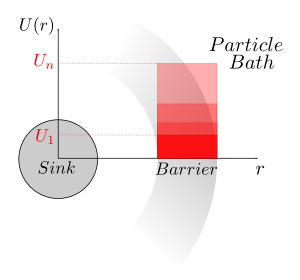
\includegraphics[width = 1.1 \textwidth]{plots/IntroSkizze.pdf}
    \caption{Sketch of system consisting of a spherical sink surrounded by a spherically symmetric step shaped barrier (indicated in \textcolor{red}{red}) embedded in a bath of Brownian particles.}
    \label{introSketch}
\end{wrapfigure}
analogy to the escape problem studied by Doering and Gadoua.
For barrier fluctuations that are fast compared to the diffusional relaxation of the Brownian particles it can be assumed that the particles move subject to a potential of mean force, such that the rate approaches that over an average barrier. For barrier fluctuations that are very slow compared to the diffusional relaxation of the particles the rate approaches the average of the rates over the different barrier configurations.
If it is not possible to separate the timescales of particle diffusion and barrier fluctuations, a more complex behavior arises. This behavior will be the main focus of this thesis. 
Other points of interest are 1) the dependence of effects on the geometry of the system and 2) the connection to experiments and simulations.

\section{Thesis Outline}
In order to be self contained an to follow a pedagogical approach, chapter \ref{Short_Introduction_to_Stochastic_Processes} gives a short introduction to stochastic processes. This is supposed to help the reader follow A) the examples from diffusion controlled reaction theory in section \ref{K_s}, \ref{The_Debye_Reaction_Rate} and B) the derivations made in section \ref{Reaction_Rates_over_Fluctuating_Barriers}. \\
Chapter \ref{numeric_model} contains two numerical methods to investigate the model and displays preliminary numeric results. \\
Chapter \ref{Reaction_Rates_over_Fluctuating_Barriers} gives an analytical treatment of a system consisting of a spherical sink surrounded by a metastable step shaped potential barrier that is embedded by a bath of Brownian particles and derives an expression for the rate of encounters of these particles with the sink. \\
Chapter \ref{results} evaluates a concrete example of the system described in chapter \ref{Reaction_Rates_over_Fluctuating_Barriers}. It analyzes the effects arising from coupling between diffusional relaxation and barrier fluctuations in terms of particle fluxes and gives a thorough study of all relevant parameters and their limits. Since it is a common procedure typically used to rationalize experimental and simulation data this chapter also studies effects that arise from the reduction of the system to only the spatial coordinates through averaging over potential fluctuations. Chapter \ref{conclusion} sums up the results and gives an outlook on further work. \\

The experienced reader may skip chapter \ref{Short_Introduction_to_Stochastic_Processes} and \ref{numeric_model} since they are basically a collection of relevant textbook knowledge and proceed directly with chapter \ref{Reaction_Rates_over_Fluctuating_Barriers} and \ref{results} which contain new and relevant results. 
